\section{Preliminaries}
\subsection{Inference Process of dLLMs}
Most recent diffusion LLMs adopt the discrete masked diffusion model paradigm \cite{mdm1, mdm2}, where generation is cast as an iterative unmasking process. Unlike autoregressive models that commit tokens sequentially, dLLMs start from a heavily masked sequence and progressively recover masked positions over several denoising steps until no \mask{} remains. At each step, the model predicts token distributions for all masked positions, conditioned on the current state.

Given a prompt $X$, we initialize the response as a fully masked sequence of predefined length $L$:
\begin{equation*}
y^{(0)} = (\mask{},\ldots,\mask{}) \in (\mathcal{V}\cup\{\mask{}\})^L .
\end{equation*}
Here, $\mathcal{V}$ denotes the vocabulary and $\mask{}$ is the special mask token. In the naive setting, the sampler unmasks exactly one token with the highest confidence per step. At each denoising step $t=0,1,\ldots, L-1$, it concatenates the prompt $X$ and the current response state $y^{(t)}$ as the model input, and commits the corresponding token at the \mask{} response position with the highest confidence:
\begin{equation*}
\begin{aligned}
c_i^{(t)} &\triangleq \max_{v\in\mathcal{V}} p_{\theta}(y_i = v \mid X, y^{(t)}), \quad i\in M^{(t)},\\
i_t &= \arg\max_{i\in M^{(t)}} c_i^{(t)},\\
y_i^{(t+1)} &=
\begin{cases}
\displaystyle \arg\max_{v\in\mathcal{V}} p_{\theta}(y_i = v \mid X, y^{(t)}), & \text{if } i=i_t,\\
y_i^{(t)}, & \text{otherwise.}
\end{cases}
\end{aligned}
\end{equation*}
% \begin{align*}
% i_t
% &= \arg\max_{i \in M^{(t)}}\! \Big( \max_{v\in\mathcal{V}}
% p_{\theta} \ (y_i = v \mid X, y^{(t)}) \Big),\\
% y_i^{(t+1)}
% &=
% \begin{cases}
% \displaystyle \arg\max_{v\in\mathcal{V}}
% p_{\theta}\!\left(y_i = v \mid X, y^{(t)}\right), & \text{if } i=i_t,\\[3pt]
% y_i^{(t)}, & \text{otherwise.}
% \end{cases}
% \end{align*}
where $M^{(t)} \triangleq \{ i \mid y^{(t)}_{i}=\mask{} \}$ denotes the set of masked response positions at step $t$. Repeating this procedure for $L$ steps yields a fully unmasked response $y^{(L)}$.

Despite the inherent parallelism within each step, practical dLLM inference exhibits a pronounced quality--speed trade-off \cite{d3llm}: directly unmasking multiple tokens in one step leads to substantial quality degradation. 
% As a result, even with the KV cache mechanism, existing dLLMs may struggle to consistently outperform strong AR baselines equipped with MTP \cite{spec, eagle3} in real scenarios.

\begin{figure*}[t!]
    \centering
    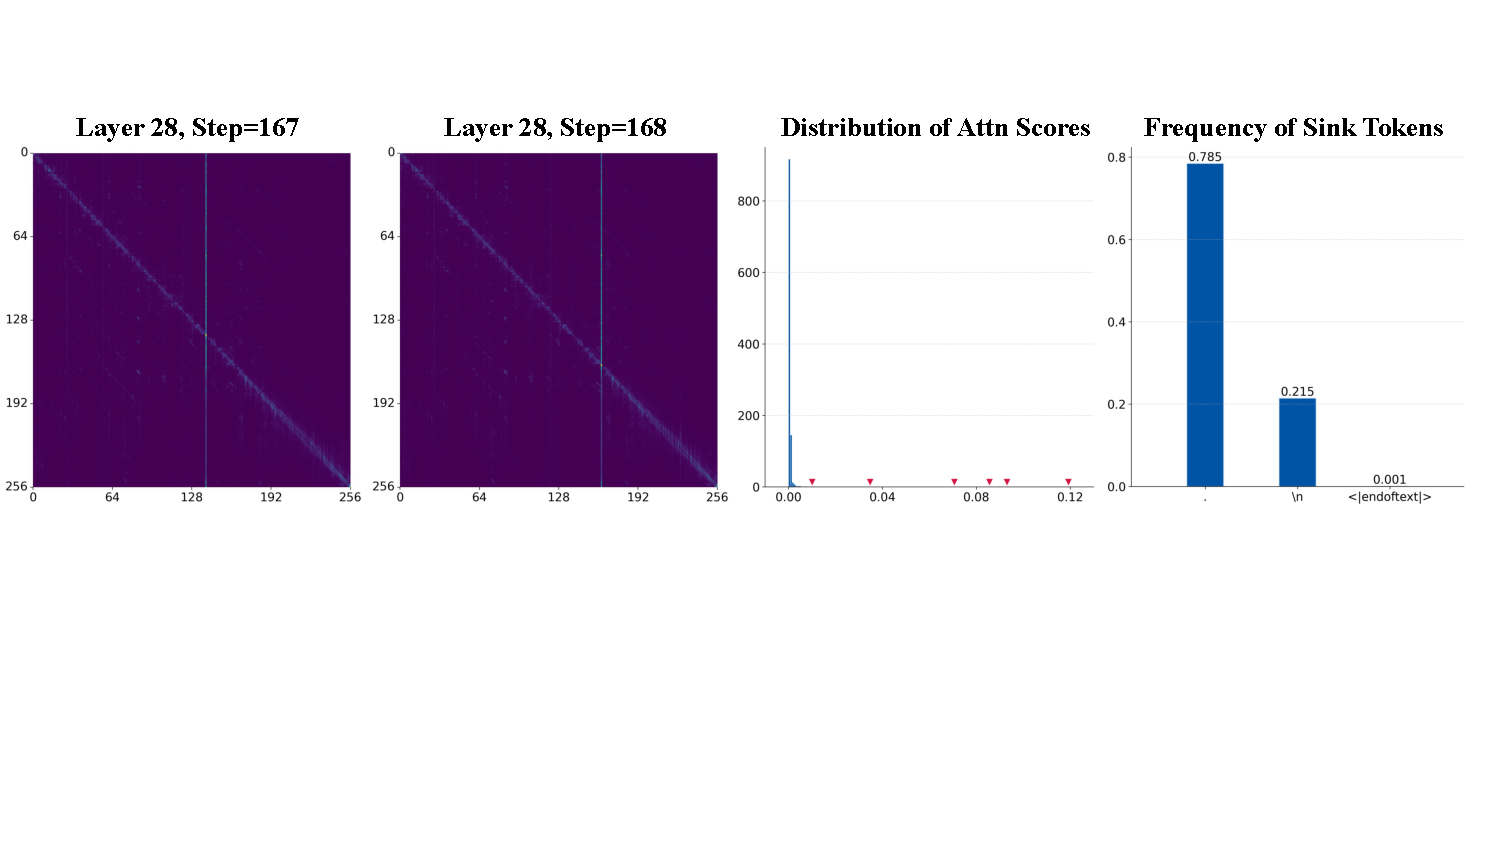
\includegraphics[width=\textwidth]{fig/attn_sink.pdf}
    \caption{\textbf{Attention Sinks in dLLMs.} We conduct experiments on multiple samples using LLaDA-8B-Instruct. Left: The two heatmaps show partial attention maps from the same layer at different denoising steps, illustrating that the attention sink shifts across denoising iterations. Right: The third plot reports the distribution of attention scores corresponding to the first plot, and the rightmost plot reports the frequency of sink tokens from multiple samples.}
    \label{fig:attn_sink}
\end{figure*}



\subsection{Nonindependent Position Predictions}\label{prl: parallel}
Unmasking a single token per step is inherently slow, and runs counter to the full position computation paradigm of dLLMs, where each denoising step produces predictions for all positions simultaneously. A common approach is to commit tokens at different positions independently according to the model’s predictive distributions at each position:
\begin{equation*}
p_{\theta}\!\left(\{y_i\}_{i\in U^{(t)}} \mid X, y^{(t)}\right) \approx \prod_{i\in U^{(t)}} p_{\theta}\!\left(y_i \mid X, y^{(t)}\right),
\end{equation*}
where $U^{(t)} \subseteq M^{(t)}$ is a set of parallel unmasking positions. However, position predictions in masked refinement are often statistically coupled. Committing multiple tokens at strongly coupled positions in the same step can introduce inconsistencies and degrade generation quality. As the classic example in prior work \cite{parallelcurse, fastdllm}, two-word poker hands (e.g., “high card,” “two pair,” “full house,” “straight flush”) must match as a pair, while parallel sampling can produce invalid combinations such as “high house”. However, if we first decode one of them like “\mask{} house”, then the probability of recovering a valid pair in the next step becomes much higher, which aligns with the conditional probability factorization: $p(y_i, y_j \mid X, y^{(t)}) = p(y_j \mid X, y^{(t)})\, p(y_i \mid y_j, X, y^{(t)})$. This nature of dLLMs suggests that parallel updates should account for position dependencies, avoiding strongly coupled positions while increasing the number of safely updated positions per step.
